
\chapter[Self-adaption \& Run-time Reconfiguration for SMC Applications]{Self-adaption and Run-time Reconfiguration for Sequential Monte Carlo Applications}

\section{Introduction}

Particle filter (PF), also known as sequential Monte Carlo (SMC) method, is a statistical method for dynamic systems involving non-linear and non-Gaussian properties. 
PF has been studied in various application areas including object tracking~\cite{happe11}, robot localisation~\cite{montemerlo02}, speech recognition~\cite{vermaak02} and air traffic management~\cite{eele11}.

PF keeps track of a large number of particles where each contains information about how a system would evolve.
The underlying concept is to approximate a sequence of states as a collection of particles.
Each particle is weighted to reflect the quality of an approximation.
The more complex the problem, the larger the number of particles that are needed.
One drawback of PF is its long execution times that limit its practical use.

This paper presents an efficient solution to PF.
We derive an adaptive algorithm that adjusts its computation complexity at run time based on the quality of results.
To map our algorithm to a heterogeneous reconfigurable system (HRS) consisting of multiple FPGAs and CPUs,
we design a pipeline-friendly data structure to make effective use of the stream computing model.
Moreover, we effectively accelerate the algorithm with a data compression scheme and data control separation.

The key contributions of this paper include:

\begin{enumerate}
\item An adaptive PF algorithm which adapts the size of particle set at run-time. 
The algorithm is able to reduce computation workload while maintaining quality of results.
\item Mapping the proposed algorithm to a scalable and reconfigurable system by following the stream computing model.
A novel data structure is designed to take advantage of the architecture and to alleviate the data transfer bottleneck.
The system uses the run-time reconfigurability of FPGA to switch between computation mode and low-power mode.
\item An implementation of a robot localisation application targeting the proposed system. 
Compared to a non-adaptive and non-reconfigurable implementation, the idle power of our proposed system is reduced by 25-34\% and the overall energy consumption decreases by 17-33\%.
Our system with four FPGAs is up to 169 times faster than a single core CPU, 41 times faster than a 1U CPU server with 12 cores, and 3 times faster than a modelled four-GPU system.
\end{enumerate}

%%%%%%%%%%%%%%%%%%%%%%%%%%%%%%%%%%%%%%%%
\section{Overview}

This section briefly outlines the PF algorithm.
A more detailed description can be found in~\cite{doucet01}. 
PF estimates the state of a system by a sampling-based approximation of the state probability density function. 
The state of a system in time-step $t$ is denoted by $X_t$. 
The control and observation are denoted by $U_t$ and $Y_t$ respectively. 
Three pieces of information about the system are known a-priori: 
\begin{itemize}
\item $p(X_0)$ is the probability of the initial state of the system, 
\item $p(X_t|X_{t-1},U_{t-1})$ is the state transition probability of the system's current state given a previous state and control information, 
\item $p(Y_t|X_t)$ is the observation model describing the likelihood of observing the measurement at the current state.
\end{itemize}

PF approximates the desired posterior probability $p(X_{t}|Y_{1:t})$ using a set of $P$ particles $\{\chi^{(i)}_t\}^P_{i=1}$ with their associated weights $\{w^{(i)}\}^P_{i=1}$. 
$X_0$ and $U_0$ are initialised.
This computation consists of three iterative steps.

\begin{enumerate}
\item \textbf{Sampling}: A new particle set $\{\widetilde{\chi}^{(i)}_t\}^P_{i=1}$ is drawn from the distribution $p(X_t|X_{t-1},U_{t-1})$, forming a prediction of the distribution of $X_t$.
\item \textbf{Importance weighting}: The likelihood $p(Y_t|\widetilde{\chi}^{(i)}_t)$ of each particle is calculated. 
The likelihood indicates whether the current measurement $Y_t$ matches the predicted state $\{\widetilde{\chi}^{(i)}_t\}^P_{i=1}$. 
Then each particle is assigned a weight $w^{(i)}$ with respect to the likelihood.
\item \textbf{Resampling}: Particles with higher weights are replicated and the number of particles with lower weights is reduced. 
With resampling, the particle set has a smaller variance. 
The particle set is used in the next time-step to predict the posterior probability subsequently. 
The distribution of the resulting particles $\{\chi^{(i)}_t\}^P_{i=1}$ approximates $p(X_t|Y_{1:t})$.
\end{enumerate}

The particles in PF are independent of each other.
It means the algorithm can be accelerated using specialised hardware with massive parallelism and pipelining.
In~\cite{happe11}, an approach for PF on a hybrid CPU/FPGA platform is developed.
Using a multi-threaded programming model, computation is switched between hardware and software during run-time to react to performance requirements. 
Resampling algorithms and architectures for distributed PFs are proposed in~\cite{bolic05}.

Adaptive PFs have been proposed to improve performance or quality of state estimation by controlling the number of particles dynamically. 
Likelihood-based adaptation controls the number of particles such that the sum of weights exceeds a pre-specified threshold~\cite{koller98}.
Kullback Leibler distance (KLD) sampling is proposed in~\cite{fox03}, which offers better quality results than likelihood-based approach. 
KLD sampling is improved in~\cite{park10} by adjusting the variance and gradient of data to generate particles near high likelihood regions. 
The above methods introduce data dependencies in the sampling and importance weighting steps, so they are difficult to be parallelised. 
An adaptive PF is proposed in~\cite{bolic02} that changes the number of particles dynamically based on estimation quality. 
In~\cite{chau12}, adaptive PF is extended to a multi-processor system on FPGA.
The number of particles and active processors change dynamically but the performance is limited by soft-core processors.
In~\cite{liu07}, a mechanism and theoretical lower bound for adapting the sample size of particles is presented.
Our previous work~\cite{chau13a} presents a hardware-friendly adaptive PF. 
The algorithm is mapped to an accelerator system which consists of an FPGA and a CPU.
However, the system suffers from a large communication overhead when the particles are transferred between the FPGA and CPU.
Moreover, the scalability of the adaptive PF algorithm to multi-FPGA is not well-studied.
In this paper, we extend our previous work to address the problems mentioned above.

%%%%%%%%%%%%%%%%%%%%%%%%%%%%%%%%%%%%%%%%
\section{Adaptive Particle Filter}
\label{sec:apf}

This section introduces an adaptive PF algorithm which changes the number of particles at each time-step.
The algorithm is inspired by~\cite{liu07} and we transform it to a pipeline-friendly version for mapping to the stream computing architecture.
This algorithm is shown in Algorithm~\ref{algo:pf} which consists of four stages.

\begin{algorithm}
\caption{Adaptive PF algorithm}
{\fontsize{8}{8}\selectfont
\begin{algorithmic}[1]
\STATE{$P_0 \gets P_{max}$}
\STATE{$\{X^{(i)}_0\}^{P_0}_{i=1} \gets $random set of particles}
\STATE{$t=1$}
\FOR{each step $t$}
	\STATE{$r=0$}
	\WHILE{$r \leq itl\_repeat$}
	{\color{gray} \STATE{---On FPGAs---}}
	\STATE{Sample a new state $\{\widetilde{\chi}_{t+1}^{(i)}\}^{P_t}_{i=1}$ from $\{\chi_{t}^{(i)}\}^{P_t}_{i=1}$} \label{algo:pf_si1}
	\STATE{Calculate unnormalised importance weights $\{\widetilde{w}^{(i)}\}^{P_t}_{i=1}$ and accumulate the weights as $w_{sum}$} \label{algo:pf_si2}
	\STATE{Calculate the lower bound of sample size $\widetilde{P}_{t+1}$ by Equation~\ref{eqt:bound2}} \label{algo:pf_lb}
	{\color{gray} \STATE{---On CPUs---}}
	\STATE{Sort $\{\widetilde{\chi}_{t+1}^{(i)}\}^{P_t}_{i=1}$ in descending $\{\widetilde{w}^{(i)}\}^{P_t}_{i=1}$} \label{algo:pf_sort}
	\IF{$\widetilde{P}_{t+1} < P_{t}$} \label{algo:pf_rd1}
		\STATE{$P_{t+1} = max\left(\lceil\widetilde{P}_{t+1}\rceil, P_{t}/2\right)$}
		\STATE{Set $a = 2P_{t+1}-P_{t}$ and $b = P_{t+1}$}
		{\color{gray} \STATE{--Do the following loop in parallel--}}
		\FOR{$i$ in $P_t-P_{t+1}$} \label{algo:pf_loop1s}
			\STATE{$\widetilde{\chi}^{(i)}_{t+1} = \frac{\chi_{t+1}^{(a)} \widetilde{w}^{(a)} + \chi_{t+1}^{(b)} \widetilde{w}^{(b)}}{\widetilde{w}^{(a)} + \widetilde{w}^{(b)}}$}
			\STATE{$\widetilde{w}^{(i)} = \widetilde{w}^{(a)} + \widetilde{w}^{(b)}$}
			\STATE{$a = a+1$ and $b = b-1$}
		\ENDFOR \label{algo:pf_rd2} \label{algo:pf_loop1e}
	\ELSIF{$\widetilde{P}_{t+1} \geq P_{t}$} \label{algo:pf_rd3}
		\STATE{$a=0$ and $b=0$}
		\FOR{$i$ in $P_{t+1}-P_{t}$}
			\IF{$\widetilde{w}^{(a)}<\widetilde{w}^{(a+1)}$ and $a<P_{t+1}$}
				\STATE{$a=a+1$}
			\ENDIF
			\STATE{$\widetilde{\chi}^{(P_{t}+b)}_{t+1} = \widetilde{\chi}^{(a)}_{t+1}/2$}
			\STATE{$\widetilde{\chi}^{(a)}_{t+1} = \widetilde{\chi}^{(a)}_{t+1}/2$}
			\STATE{$\widetilde{w}^{(P_{t}+b)} = \widetilde{w}^{(a)}/2$}
			\STATE{$\widetilde{w}^{(a)} = \widetilde{w}^{(a)}/2$}
			\STATE{$b=b+1$}
		\ENDFOR
	\ENDIF \label{algo:pf_rd4}
	\STATE{Resample $\{\widetilde{\chi}^{(i)}_{t+1}\}^{P_t}_{i=1}$ to $\{\chi^{(i)}_{t+1}\}^{P_{t+1}}_{i=1}$} \label{algo:pf_r}
	\STATE{$r=r+1$}
	\ENDWHILE
\ENDFOR
\end{algorithmic}
}
\label{algo:pf}
\end{algorithm}

\subsection{Stage 1: Sampling and Importance Weighting (line~\ref{algo:pf_si1} to~\ref{algo:pf_si2})}
At the initial time-step ($t=0$), the maximum number of particles are used, i.e. $P_0=P_{max}$.
At the subsequent time-steps, the number of particles is denoted as $P_{t}$.
Initially, the particle set $\{\chi_{t}^{(i)}\}^{P_t}_{i=1}$ is sampled to $\{\widetilde{\chi}_{t+1}^{(i)}\}^{P_t}_{i=1}$.
Then a weight from $\{w^i\}^{P_t}_{i=1}$ is assigned to each particle. 
As a result, $\{\widetilde{\chi}_{t+1}^{(i)}\}^{P_t}_{i=1}$ and $\{w^{(i)}\}^{P_t}_{i=1}$ give an estimation of the next state.

During sampling and importance weighting, the computation of every particle is independent of each other. 
The mapping of computation to FPGAs will be described in Section~\ref{sec:hrs}.

\subsection{Stage 2: Lower Bound Calculation (line~\ref{algo:pf_lb})} 
This stage derives the smallest number of particles that are needed in the next time-step in order to bound the approximation error.
The adaptive algorithm seeks a value which is less than or equal to $P_{max}$.
This number, denoted as $\widetilde{P}_{t+1}$, is referred to as the lower bound of sampling size.
It is calculated by Equation~\ref{eqt:bound2} to ~\ref{eqt:bound5}.

\begin{equation}
\small
\begin{aligned}
\widetilde{P}_{t+1} = \sigma^2 \cdot \frac{P_{max}}{Var(\{\widetilde{\chi}_{t+1}^{(i)}\}^{P_t}_{i=1})}
\end{aligned}
\label{eqt:bound2}
\end{equation}

\begin{eqnarray}
\small
\begin{aligned}
\sigma^2 = & \sum_{i=1}^{P_{t}}\left({w}^{(i)} \cdot \widetilde{\chi}_{t+1}^{(i)} \right)^2 - 2 \cdot E(\{\widetilde{\chi}_{t+1}^{(i)}\}^{P_t}_{i=1}) \cdot \sum_{i=1}^{P_{t}} \left ( ({w}^{(i)})^2 \cdot \widetilde{\chi}_{t+1}^{(i)} \right ) \\
& + \left(E(\{\widetilde{\chi}_{t+1}^{(i)}\}^{P_t}_{i=1})\right)^2 \cdot \sum_{i=1}^{P_{t}}({w}^{(i)})^2
\end{aligned}
\label{eqt:bound3}
\end{eqnarray}

\begin{equation}
\small
\begin{aligned}
Var(\{\widetilde{\chi}_{t+1}^{(i)}\}^{P_t}_{i=1}) = \sum_{i=1}^{P_{t}} \left ( {w}^{(i)} \cdot (\widetilde{\chi}_{t+1}^{(i)})^2 \right ) - \left( E(\{\widetilde{\chi}_{t+1}^{(i)}\}^{P_t}_{i=1}) \right)^2
\end{aligned}
\label{eqt:bound4}
\end{equation}

\begin{equation}
\small
\begin{aligned}
E(\{\widetilde{\chi}_{t+1}^{(i)}\}^{P_t}_{i=1}) = \sum_{i=1}^{P_{t}} {w}^{(i)} \cdot \widetilde{\chi}_{t+1}^{(i)}
\end{aligned}
\label{eqt:bound5}
\end{equation}

As shown in Equation~\ref{eqt:bound3} to \ref{eqt:bound5}, ${w}^{(i)}$ is a normalised term. 
To calculate $w^{(i)}$, a traditional software-based approach is to iterate through the set of particles twice.
The sum of weights $w_{sum}$ and unnormalised weight $\widetilde{w}^{(i)}$ are calculated in the first iteration.
Then $w^{(i)}$ is obtained by dividing $\widetilde{w}^{(i)}$ by $w_{sum}$ in the second iteration.
However, this method is inefficient for FPGA implementation.
Since $2P_t$ cycles are needed to process $P_t$ pieces of data, the throughput is reduced to 50\%.

To fully utilise the deep pipeline on FPGA, we perform function transformation.
Given ${w}^{(i)} = \frac{\widetilde{w}^{(i)}}{w_{sum}}$, we extract $w_{sum}$ out of Equation~\ref{eqt:bound3} to \ref{eqt:bound5}.
By doing so, we obtain a transformed form as shown in Equations~\ref{eqt:bound6} to~\ref{eqt:bound8}.
$w_{sum}$ and $\widetilde{w}^{(i)}$ are computed simultaneously in two separate data paths.
At the last clock cycle of the particle stream, $\sigma^2$, $Var(\{\widetilde{\chi}_{t+1}^{(i)}\}^{P_t}_{i=1})$ and $E(\{\widetilde{\chi}_{t+1}^{(i)}\}^{P_t}_{i=1})$ are obtained.
The details of the FPGA kernel design will be explained in Section~\ref{sec:hrs}.

\begin{eqnarray}
\small
\begin{aligned}
\sigma^2 = & \frac{1}{(w_{sum})^2} \cdot ( \sum_{i=1}^{P_{t}}\left(\widetilde{w}^{(i)} \cdot \widetilde{\chi}_{t+1}^{(i)} \right)^2 - 2 \cdot E(\{\widetilde{\chi}_{t+1}^{(i)}\}^{P_t}_{i=1}) \cdot \sum_{i=1}^{P_{t}} \left ( (\widetilde{w}^{(i)})^2 \cdot \widetilde{\chi}_{t+1}^{(i)} \right )\\
& + \left(E(\{\widetilde{\chi}_{t+1}^{(i)}\}^{P_t}_{i=1})\right)^2 \cdot \sum_{i=1}^{P_{t}}(\widetilde{w}^{(i)})^2 )
\end{aligned}
\label{eqt:bound6}
\end{eqnarray}

\begin{equation}
\small
\begin{aligned}
Var(\{\widetilde{\chi}_{t+1}^{(i)}\}^{P_t}_{i=1}) = \frac{1}{w_{sum}} \cdot \sum_{i=1}^{P_{t}} \left ( \widetilde{w}^{(i)} \cdot (\widetilde{\chi}_{t+1}^{(i)})^2 \right ) - \left( E(\{\widetilde{\chi}_{t+1}^{(i)}\}^{P_t}_{i=1}) \right)^2
\end{aligned}
\label{eqt:bound7}
\end{equation}

\begin{equation}
\small
\begin{aligned}
E(\{\widetilde{\chi}_{t+1}^{(i)}\}^{P_t}_{i=1}) = \frac{1}{w_{sum}} \cdot \sum_{i=1}^{P_{t}} \widetilde{w}^{(i)} \cdot \widetilde{\chi}_{t+1}^{(i)}
\end{aligned}
\label{eqt:bound8}
\end{equation}

\subsection{Stage 3: Particle set size tuning (line~\ref{algo:pf_sort} to~\ref{algo:pf_rd4})} 
The adaptive approach tunes the particle set size to fit the lower bound $P_{t+1}$.
This stage is done on the CPUs because the operations involve non-sequential data access that cannot be mapped efficiently to FPGAs.

The particles are sorted in descending order according to their weights.
As the new sample size can increase or decrease, there are two cases:

\begin{itemize}
\item {\bf Case I: Particle set reduction when $\widetilde{P}_{t+1} < P_{t}$} 

The lower bound $P_{t+1}$ is set to $max\left(\lceil\widetilde{P}_{t+1}\rceil, P_{t}/2\right)$.
Since the new size is smaller than the old one, some particles are combined to form a smaller particle set.
Figure~\ref{fig:tuning} illustrates the idea of particle reduction.
The first $2P_{t+1}-P_{t}$ particles with higher weights are kept and the remaining $2(P_{t}-P_{t+1})$ particles are combined in pairs.
As a result, there are $P_{t}-P_{t+1}$ new particles injected to form the target particle set with $P_{t+1}$ particles.
We combine the particles deterministically to keep the statements in the loop independent of each other.
As a result, loop unrolling is undertaken to execute the statements in parallel.
The complexity of the loop is in $\bigO{\frac{P_{t}-P_{t+1}}{N_{parallel}}}$, where $N_{parallel}$ indicates the level of parallelism.

\setcounter{subfigure}{0}
\begin{figure}[t!]
\centering
\subfigure[Combining the last $2(P_{t}-P_{t+1})$ particles with lower weights]{
\includegraphics[width=0.45\textwidth]{runtime_reconfiguration/figures/fig_tuning1} \hfill
\label{fig:tuning1}
}
\subfigure[$P_{t+1}$ new particles are formed]{
\includegraphics[width=0.45\textwidth]{runtime_reconfiguration/figures/fig_tuning2}
\label{fig:tuning2}
}
\caption{Particle set reduction}
\label{fig:tuning}
\end{figure}

\item {\bf Case II: Particle set expansion when $\widetilde{P}_{t+1} \geq P_{t}$}

The lower bound $P_{t+1}$ is set to $\widetilde{P}_{t+1}$.
Some particles are taken from the original set and are inserted to form a larger set.
The particles with larger weight would have more descendants.
As shown in line~\ref{algo:pf_rd3} to~\ref{algo:pf_rd4}, the process requires picking the particle with the largest weight at each iteration of particle incision.
Since the particle set is pre-sorted, the complexity of particle set expansion is $\bigO{P_{t+1}-P_{t}}$.

\end{itemize}

\subsection{Stage 4: Resampling (line~\ref{algo:pf_r})}
Resampling is performed to pick $P_{t+1}$ particles from $\{\widetilde{\chi}_{t+1}^{(i)}\}^{P_t}_{i=1}$ to form $\{\chi_{t+1}^{(i)}\}^{P_{t+1}}_{i=1}$.
The process has a complexity of $\bigO{P_{t+1}}$.

%%%%%%%%%%%%%%%%%%%%%%%%%%%%%%%%%%%%%%%%
\section{Heterogeneous Reconfigurable System}
\label{sec:hrs}

This section describes the proposed heterogeneous reconfigurable system (HRS).
It is scalable to cope with different FPGA devices and applications.
HRS also takes advantage of the run-time reconfiguration feature for power and energy reduction.

\subsection{Mapping adaptive PF to HRS}
\label{sec:arch}

The system design of HRS is shown in Figure~\ref{fig:arch}.
A heterogeneous structure is employed to make use of multiple FPGAs and CPUs.
FPGAs and CPUs communicate through high bandwidth buses.
FPGAs are responsible for (1) sampling, (2) importance weighting, and (3) lower bound calculation.
The data paths on the FPGAs are fully-pipelined.
Each FPGA has its own on-board dynamic random-access memory (DRAM) to store the large amount of particle data.
On the other hand, the CPUs gather all the particles from FPGAs to perform particle set size tuning and resampling.

\begin{figure}[t!]
\centering
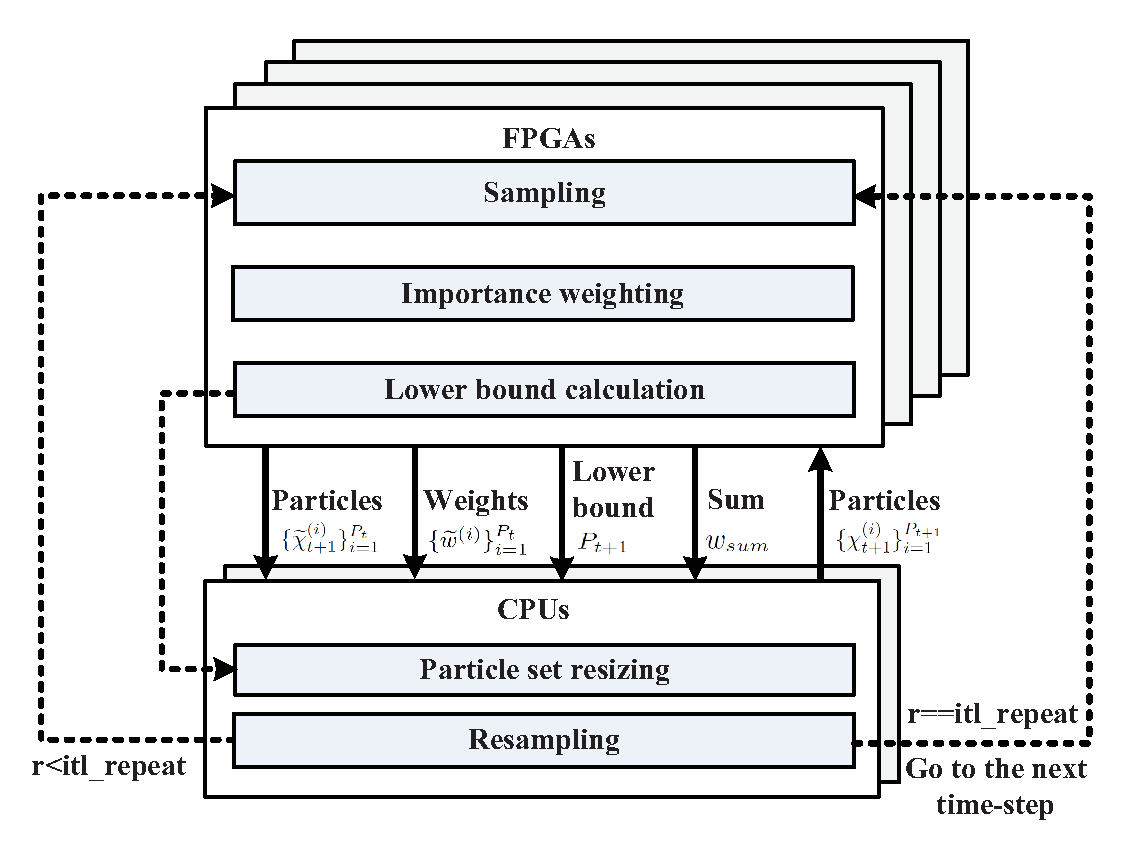
\includegraphics[width=0.7\textwidth]{runtime_reconfiguration/figures/fig_arch}
\caption{Heterogeneous reconfigurable system (Solid lines: data paths; Dotted lines: control paths)}
\label{fig:arch}
\end{figure}

\begin{figure}[t!]
\centering
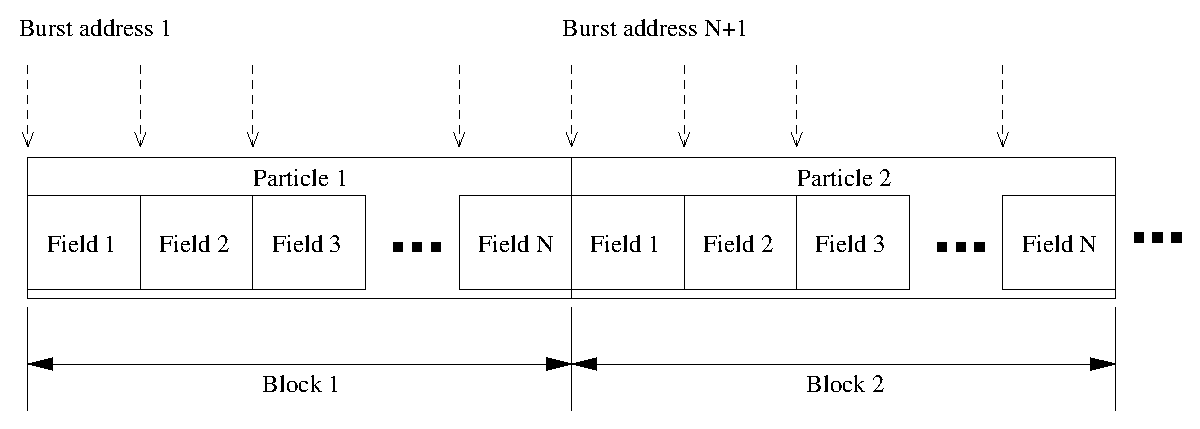
\includegraphics[width=0.8\textwidth]{runtime_reconfiguration/figures/fig_particles}
\caption{A particle stream}
\label{fig:particles_stream}
\end{figure}

\subsection{FPGA Kernel Design}
Sampling, importance weighting and lower bound calculation are the most computation intensive stages.
In each time-step, these three stages are iterated for $itl\_repeat$ times.
An FPGA kernel is designed to enable acceleration of them.

Figure~\ref{fig:kernel} shows the components of the FPGA kernel.
The kernel is fully pipelined to achieve one output per clock cycle.
It can also be replicated as many times as FPGA resource allow and the replications can be split across multiple FPGA boards.
The kernel takes three inputs from the CPUs or on-board DRAM: (1) states, (2) controls, and (3) seeds.
Application specific parameters are stored in ROMs.
Three building blocks correspond to the sampling, importance weighting and lower bound calculation stages as described in Section~\ref{sec:apf}.

For sampling and importance weighting, the computation of each particle is independent of each other.
Particles are fed to the FPGAs as a stream shown in Figure~\ref{fig:particles_stream}.
Each block of the particle stream consists of a number of data fields which store information of a particle.
The number of data fields is application dependent.
In every clock cycle, one piece of data is transferred from the onboard memory to an FPGA data path.
Each FPGA data path has a long pipeline where each stage is filled with a piece of data, and therefore many particles are processed simultaneously.
Fixed-point data representation is customised at each pipeline stage to reduce the resource usage.

Meanwhile, the accumulation of $w_{sum}$ introduces a feedback loop.
A new weight comes along every cycle which is more quickly than the floating-point unit to perform addition of the previous weight.
In order to achieve one result per clock cycle, fixed-point data-path is implemented while ensuring no overflow or underflow occurs.

\begin{figure}[t!]
\centering
\includegraphics[width=0.5\textwidth,height=130mm]{runtime_reconfiguration/figures/fig_kernel}
\caption{FPGA kernel design}
\label{fig:kernel}
\end{figure}

\subsection{Timing model for run time reconfiguration}
\label{sec:reconfig}

We derive a model to analyse the computation time of HRS.
The model helps us to design a configuration schedule that satisfies the real-time requirement and, if necessary, amend the application's specification.
The model will be validated by experiments in Section~\ref{sec:results}.

The computation time ($T_{comp}$) of HRS consists of three components: (1) Data path time $T_{datapath}$, (2) CPU time $T_{CPU}$, and (3) Data transfer time $T_{tran}$.
The sampling, importance weighting and resampling processes are repeated for $itl\_repeat$ times in every time-step.

\begin{equation}
\small
\begin{aligned}
T_{comp} = itl\_repeat \cdot \left ( T_{datapath} + T_{CPU} + T_{tran} \right )
\end{aligned}
\label{eqt:total}
\end{equation}

\textbf{Data path time}, $T_{datapath}$, denotes the time spent on the FPGAs.
$P_t$ denotes the number of particles at the current time-step and $f_{FPGA}$ denotes the clock frequency of the FPGAs.
$L$ is the length of the pipeline.
$N_{datapath}$ denotes the number of data paths on one FPGA board.
$N_{FPGA}$ is the number of FPGA boards in the system.

\begin{equation}
\small
\begin{aligned}
T_{datapath} = \left(\frac{P_t}{f_{FPGA} \cdot N_{datapath}} + L - 1 \right) \frac{1}{N_{FPGA}}
\end{aligned}
\label{eqt:kernel}
\end{equation}

\textbf{CPU time}, $T_{CPU}$, denotes the time spent on the CPUs.
The clock frequency and number of threads of the CPUs are represented by $f_{CPU}$ and $N_{thread}$ respectively.
$par$ is an application-specific parameter in the range of $[0,1]$ which represents the ratio of CPU instructions that are parallelisable, and $\alpha$ is a scaling constant derived empirically.

\begin{equation}
\small
\begin{aligned}
T_{CPU} = \alpha \cdot \frac{P_t}{f_{CPU}} \cdot \left(1-par+\frac{par}{N_{thread}}\right)
\end{aligned}
\label{eqt:host}
\end{equation}

\textbf{Data transfer time}, $T_{tran}$, denotes the time of moving a particle stream between the FPGAs and the CPUs.
$df$ is the number of data fields of a particle.
For example, if a particle contains the information of coordinates ($x$, $y$) and heading $h$, $df=3$.
Given that the constant 1 represents the weight and the constant 2 accounts for the movement of data in and out of the FPGAs,
and $bw_{data}$ is the bit-width of one data field, the expression $(2 \cdot df + 1) \cdot bw_{data}$ is regarded as the size of a particle.

$f_{bus}$ is the clock frequency of the bus connecting the CPUs to FPGAs and $lane$ is the number of bus lanes connected to one FPGA.
Since many buses, such as the PCI Express Bus, encode data during transfer, the effective data are denoted by $eff$ (in PCI Express Gen2 the value is 8/10).
In our previous work~\cite{chau13a}, the data transfer time has a significant performance impact on HRS.
To reduced the data transfer overhead, we introduce a data compression technique that will be described in Section~\ref{sec:stream}.

\begin{equation}
\small
\begin{aligned}
T_{tran} = \frac{(2 \cdot df + 1) \cdot bw_{data} \cdot P_t}{f_{bus} \cdot lane \cdot eff \cdot N_{FPGA}}
\end{aligned}
\label{eqt:data}
\end{equation}

In real-time applications, each time-step is fixed and is known as the real-time bound $T_{rt}$.
The derived model helps system designers to ensure that the computation time $T_{comp}$ is shorter than $T_{rt}$.
An idle time $T_{idle}$ is introduced to represent the time gap between the computation time and real-time bound.

\begin{equation}
\small
\begin{aligned}
T_{idle} = T_{rt} - T_{comp}
\end{aligned}
\label{eqt:idle}
\end{equation}

Figure~\ref{fig:timing1} illustrates the power consumption of HRS without run-time reconfiguration.
It shows that the FPGAs are still drawing power after the computation finishes.
By exploiting run-time reconfiguration as shown in Figure~\ref{fig:timing2}, the FPGAs are loaded with a low-power configuration during the idle period.
Such configuration minimises the amount of active resources and clock frequency.
Equation~\ref{eqt:sleep} describes the sleep time when the FPGAs are idle and being loaded with the low-power configuration.
If the sleep time is positive, reconfiguration would be helpful in these situations.

\begin{equation}
\small
\begin{aligned}
T_{sleep} = T_{idle} - T_{config}
\end{aligned}
\label{eqt:sleep}
\end{equation}

\textbf{Configuration time}, $T_{config}$, denotes the time needed to download a configuration bit-stream to the FPGAs.
$size_{bs}$ represents the size of bitstream in bits.
$f_{config}$ is the configuration clock frequency in Hz and $bw_{config}$ is the width of the configuration port.

\begin{equation}
\small
\begin{aligned}
T_{config} = \frac{size_{bs}}{f_{config} \cdot bw_{config}}
\end{aligned}
\label{eqt:cf}
\end{equation}

\setcounter{subfigure}{0}
\begin{figure}[t!]
\centering
\subfigure[Without reconfiguration]{
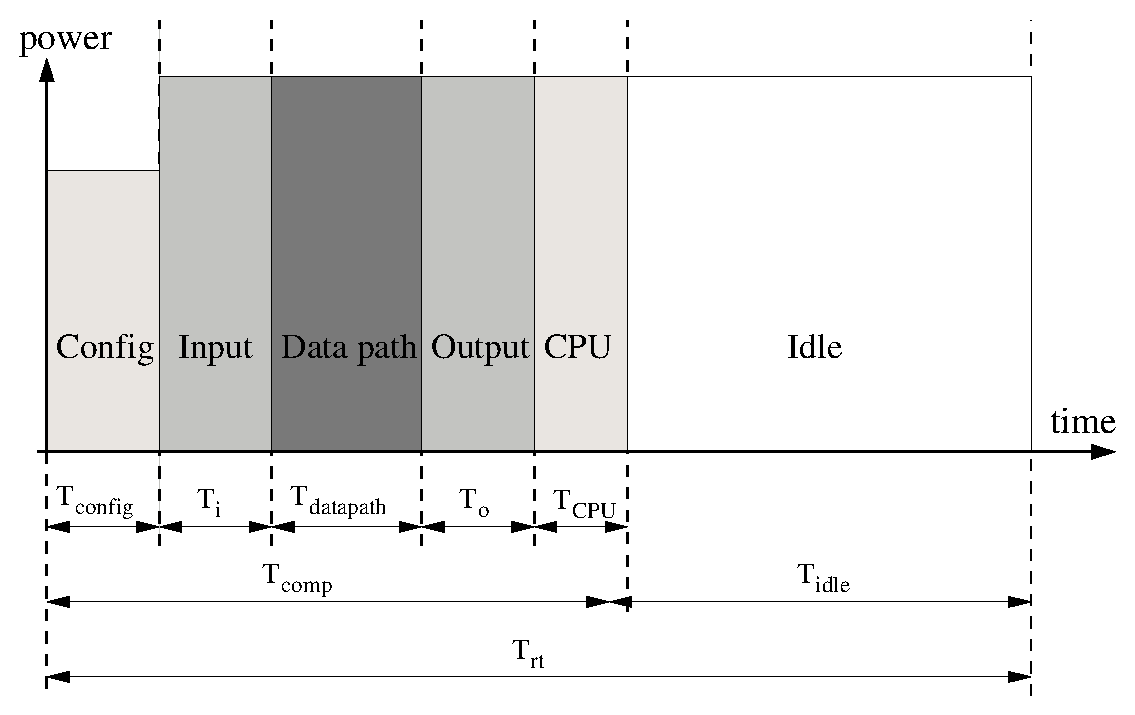
\includegraphics[width=0.6\textwidth]{runtime_reconfiguration/figures/fig_timing1} \hfill
\label{fig:timing1}
}
\subfigure[With reconfiguration to low-power mode during idle]{
\includegraphics[width=0.6\textwidth]{runtime_reconfiguration/figures/fig_timing2}
\label{fig:timing2}
}
\caption{Power consumption of the HRS over time}
\label{fig:timing}
\end{figure}

%%%%%%%%%%%%%%%%%%%%%%%%%%%%%%%%%%%%%%%%
\section{Optimising Transfer of Particle Stream}
\label{sec:stream}

In Section~\ref{sec:hrs}, the data transfer time depends on the number of particles and the bus bandwidth between the CPUs and FPGAs.
It can be a major performance bottleneck as depicted in~\cite{chau13a}.
Refer to Figure~\ref{fig:particles_resampling_unopt}, each block stores the data of a particle.
When the CPUs finish processing, all data are transferred from the CPUs to the FPGAs.
The data transfer time cannot be reduced by implementing more FPGA data paths or increasing the FPGAs' clock frequency because the bottleneck is at the bus connecting the CPUs and FPGAs.

To improve the data transfer performance, we design a data structure which facilitates compression of particles.
The idea comes from an observation of the resampling process - some particles are eliminated and the vacancies are filled by replicating non-eliminated particles.
Replication means data redundancy exists.
For example, in the original data structure shown in Figure~\ref{fig:particles_resampling_unopt}, 
particle~1 has three replicates and particle~2 is eliminated, therefore, particle~1 is stored and transferred for three times.

By using the data structure in Figure~\ref{fig:particles_resampling_opt}, data redundancy is eliminated by storing every particle once.
Each particle is also transferred once.
As a result, the data transfer time and memory space are reduced.

\setcounter{subfigure}{0}
\begin{figure}[t!]
\centering
\subfigure[Particle stream before compression]{
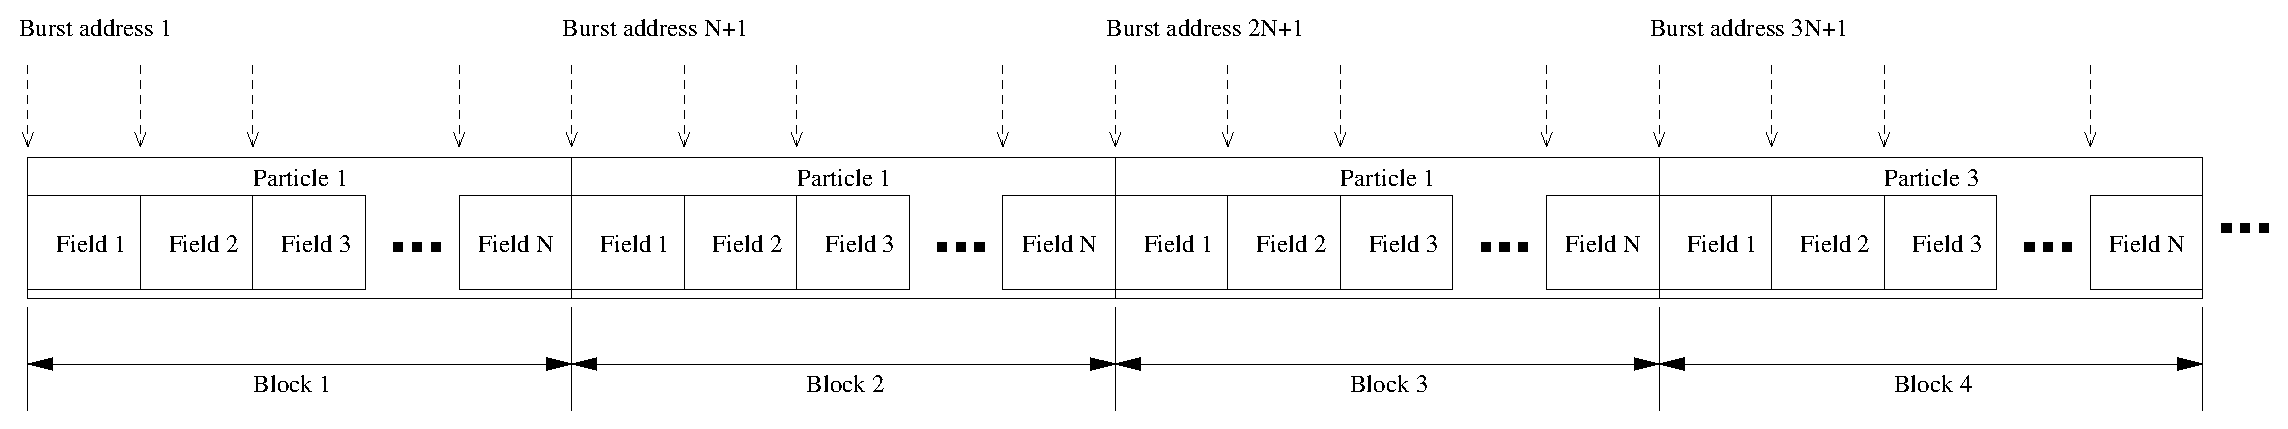
\includegraphics[width=\textwidth]{runtime_reconfiguration/figures/fig_particles_resampling}
\label{fig:particles_resampling_unopt}
}
\subfigure[Compressed particle stream]{
\includegraphics[width=\textwidth]{runtime_reconfiguration/figures/fig_particles_resampling_b}
\label{fig:particles_resampling_opt}
}
\caption{After the resampling process, some particles are eliminated and the remaining particles are replicated. Data compression is applied so that every particle is stored and transferred once only.}
\label{fig:particles_resampling}
\end{figure}

A HRS often contains DRAM which transfers data in burst in order to maximise the memory bandwidth.
This works fine with the original data structure where the data are organised as a sequence from the lower address space to the upper.
However, using the new data structure, the data access pattern is not sequential anymore, the address can go back and forth.
The DRAM controller needs to be modified so that the transfer throughput would not be affected by the change of data access pattern.
As illustrated in Figure~\ref{fig:particles_resampling_opt}, a tag sequence is used to indicate the address of the next block.
For example, after reading the data of particle~1, the burst address is at $N$.
If the tag is one, the next burst address will point to the address of the next block at $N+1$.
Otherwise, the burst address will point to the start address of the current block (which is $1$).
The data are still addressed in burst so the performance is not degraded.

The data transfer time with compression is shown below. 
$Rep$ is the average number of replication of the particles,
and therefore the size of the resampled particle stream is reduced by a ratio of $Rep$.
The range of $Rep$ is from 1 to $P_t$, depending on the distribution of particles after the resampling process.
The effect of $Rep$ on data transfer time will be evaluated in the next section.

\begin{equation}
\small
\begin{aligned}
T_{tran} = \frac{(\frac{df}{Rep} + df + 1) \cdot bw_{data} \cdot P_t}{f_{bus} \cdot lane \cdot eff \cdot N_{FPGA}}
\end{aligned}
\label{eqt:data_opt}
\end{equation}

%%%%%%%%%%%%%%%%%%%%%%%%%%%%%%%%%%%%%%%%
\section{Experimental Results}
\label{sec:results}

To evaluate the performance of the HRS and make comparison with the other systems, 
we implement an application which uses PF for localisation and tracking of mobile robot.
The application is proposed in~\cite{montemerlo02} to track location of moving objects conditioned upon robot poses over time.
Given a priori learned map, a robot receives sensor values and moves at regular time intervals. 
Meanwhile, $M$ moving objects are tracked by the robot.
The states of the robot and objects at time $t$ are represented by a state vector $X_t$:
 
\begin{equation}
\small
\begin{aligned}
X_t = \{R_t, H_{t,1}, H_{t,2}, ..., H_{t,M}\}
\end{aligned}
\end{equation}

$R_t$ denotes the robot's pose at time $t$, and $H_{t,1}, H_{t,2}, ..., H_{t,M}$ denote the locations of the $M$ objects at the same time.

The following equation is used to represent the posterior of the robot's location:

\begin{equation}
\small
\begin{aligned}
p(X_t|Y_t,U_t) = p(R_t|Y_t,U_t) \prod_{m=1}^M p(H_{t,m}|R_t,Y_t,U_t)
\end{aligned}
\end{equation}

$Y_t$ is the sensor measurement and $U_t$ is the control of the robot at time $t$.
The robot path posterior $p(R_t|Y_t,U_t)$ is represented by a set of robot-particles.
The distribution of an object's location $p(H_{t,m}|R_t,Y_t,U_t)$ is represented by a set of object-particles, where each object-particle set is attached to one particular robot-particle.
In other words, if there are $P_r$ robot-particles representing the posterior over robot path, there are $P_r$ object-particle sets, each has $P_h$ particles.

In the application, the area of the map is 12m by 18m.
The robot makes a movement of 0.5m every five seconds, i.e. $T_{rt} = 5$.
The robot can track eight moving objects at the same time.
A maximum of 8192 particles are used for robot-tracking and each robot-particle is associated with 1024 object-particles.
Therefore, the maximum number of data path cycles is 8*8192*1024=67,108,864.
Each particle being streamed into the FPGAs contains coordinates ($x$,$y$) and heading $h$ which are represented by three single precision floating-point numbers.
For the particle being streamed out of the FPGAs, it also contains a weight in addition to the coordinates.
From Equation~\ref{eqt:data}, the size of a particle is $(2 \cdot 3 + 1) \cdot 32 \mbox{ bits} = 224 \mbox{ bits}$.

\subsection{System Settings}

\textbf{HRS}: Two reconfigurable accelerator systems from Maxeler Technologies are used.
The system is developed using MaxCompiler, which adopts a stream computing model.
\begin{itemize}
\item \textit{MaxWorkstation} is a microATX form factor system which is equipped with one Xilinx Virtex-6 XC6VSX475T FPGA.
The FPGA has 297,600 lookup tables (LUTs), 595,200 flip-flops (FFs), 2,016 digital signal processors (DSPs) and 1,064 block RAMs. 
The FPGA board is connected to an Intel i7-870 CPU (4 physical cores, 8 threads in total, clocked at 2.93 GHz) via a PCI Express Gen2 x8 bus.
The maximum bandwidth of the PCI Express bus is 2 GB/s according to the specification provided by Maxeler Technologies.
\item \textit{MPC-C500} is a 1U server accommodating four FPGA boards, each of which has a Xilinx Virtex-6 XC6VSX475T FPGA.
Each FPGA board is connected to two Intel Xeon X5650 CPUs (12 physical cores, 24 threads in total, clocked at 2.66 GHz) via a PCI Express Gen2 x8 bus.
\end{itemize}

To support run-time reconfigurability, there are two FPGA configurations:
\begin{itemize}
\item {\it Sampling and importance weighting configuration} is clocked at 100 MHz.
Two data paths are implemented on one FPGA to process particles in parallel.
The total resource usage is 231,922 LUTs (78\%), 338,376 FFs (56\%), 1,934 DSPs (96\%) and 514 block RAMs (48\%).
\item {\it Low-power configuration} is clocked at 10 MHz, with 5,962 LUTs (2\%), 6,943 FFs (1\%) and 12 block RAMs (1\%).
It uses minimal resources just to maintain communication between the FPGAs and CPUs.
\end{itemize}

\textbf{CPU}: The CPU performance results are obtained from a 1U server that hosts two Intel Xeon X5650 CPUs. 
Each CPU is clocked at 2.66 GHz.
The program is written in C language and optimised by Intel Compiler with SSE4.2 and flag {\it -fast} enabled.
OpenMP is used to utilise all the processor cores.

\textbf{GPU}: An NVIDIA Tesla C2070 GPU is hosted inside a 4U server.
It has 448 cores running at 1.15 GHz and has a peak performance by 1288 GFlops.
The program is written in C for CUDA and optimised to use all the cores available.
To get more comprehensive results for comparison, we also estimate the performance of multiple GPUs.
The estimation is based on the fact that the first three stages (sampling, importance weighting, lower bound calculation) can be evenly distributed to every GPU and be computed independently, 
so the data path and data transfer speedup scales linearly with the number of GPUs.
On the other hand, the last two stages (particle set resizing, resampling) are computed on the CPU no matter how many GPUs are used, therefore, the CPU time does not scale with the number of GPUs.

\subsection{Adaptive PF versus Non-adaptive PF}
The comparison of adaptive and non-adaptive PF is shown in Table~\ref{tab:pf}.
Both model estimation and experimental results are listed.
Initially, the maximum number of particles are instantiated for global localisation.
For the non-adaptive scheme, the particle set size does not change.
The total computation time estimated and measured are 1.328 seconds and 1.885 seconds, respectively.
The difference is due to the difference between the effective and maximum bandwidth of the PCI Express bus.

\begin{table}[h]
	\setlength{\tabcolsep}{5pt}
	\begin{spacing}{1.0}
	\caption{Comparison of adaptive and non-adaptive PF on HRS (MaxWorkstation with one FPGA, no data compression is applied)\label{tab:pf}}{
	\centering
	\smallskip
		\begin{tabular}{| l || c c | c c |}
			\hline
			 \multirow{2}{*}{}  & \multicolumn{2}{|c|}{Non-adaptive PF} & \multicolumn{2}{|c|}{Adaptive PF} \\
			\hline
			  & Model & Exp. & Model & Exp. \\
			\hline
			\hline
			 No. of particles & \multicolumn{2}{|c|}{67M} & \multicolumn{2}{|c|}{573k} \\
			\hline
			 Data path time $T_{datapath}$ (s) 		& 0.336 & 0.336 & 0.003 & 0.003 \\
			 CPU time $T_{CPU}$ (s) 				& 0.117 & 0.117 & 0.001 & 0.001 \\
			 Data time $T_{tran}$ (s) 				& 0.875 & 1.432 & 0.007 & 0.012 \\
			 Total comp. time $T_{comp}$ (s)			& 1.328 & 1.885 & 0.011	& 0.016 \\
			\hline
			 Comp. speedup (higher is better)		& 1x	& 1x	& 120.7x	& 117.8x \\
			\hline
		\end{tabular}
	}
	\end{spacing}
\end{table}

For the adaptive scheme, the number of particles varies from 573k to 67M, and the computation time scales linearly with the number of particles.
From Table~\ref{tab:pf}, both the model and experiment show 99\% reduction in computation time.

Figure~\ref{fig:adaptive} shows how the number of particles and the components of total computation time vary over the wall-clock time (passage of time from the start to the completion of the application).
Although the number of particles is reduced in the proposed design, the results in Figure~\ref{fig:error} show that the localisation error is not adversely affected.
The error is the highest during initial global localisation and it is reduced when the robot moves.

\begin{figure}[t!]
\centering
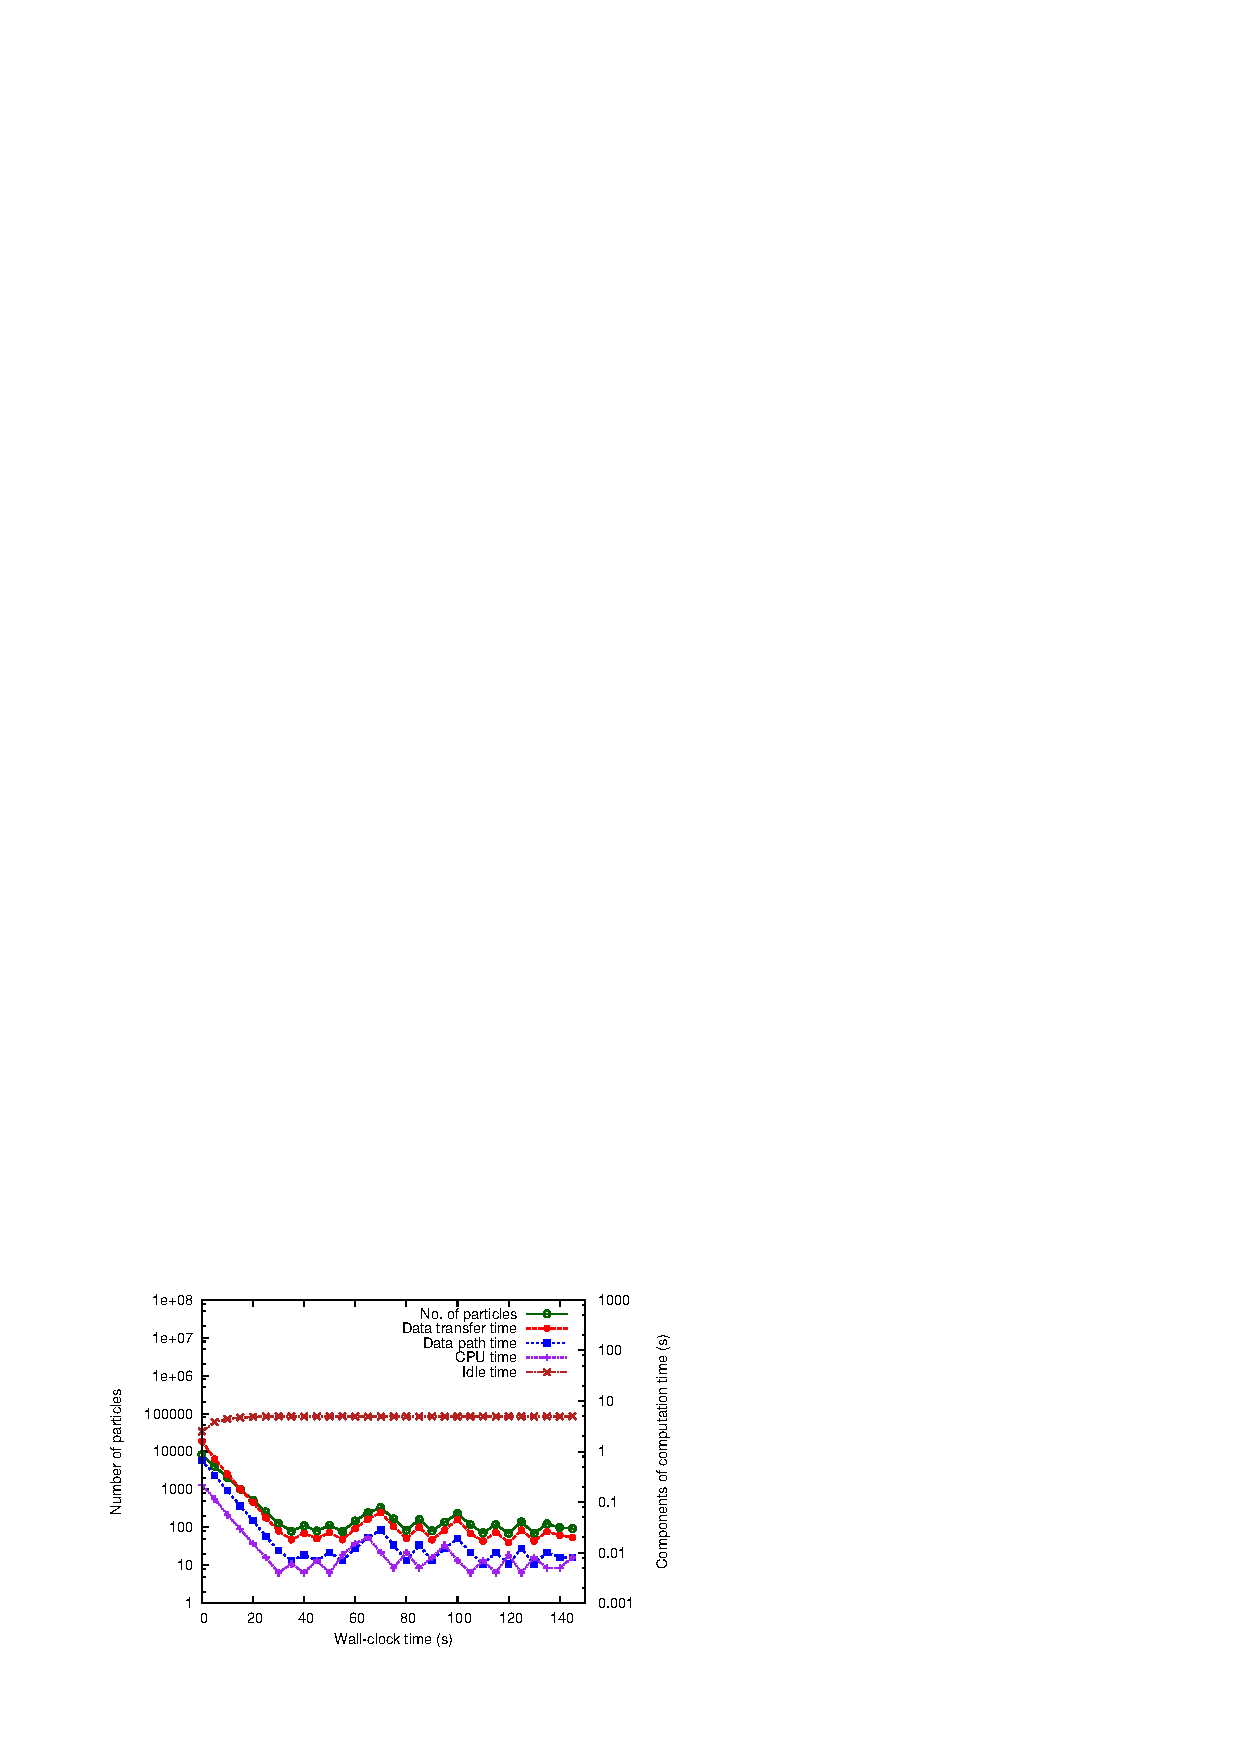
\includegraphics[width=0.7\textwidth]{runtime_reconfiguration/figures/fig_adaptive}
\caption{Number of particles and components of total computation time versus wall-clock time}
\label{fig:adaptive}
\end{figure}

\begin{figure}[t!]
\centering
\includegraphics[width=0.7\textwidth]{runtime_reconfiguration/figures/fig_error}
\caption{Localisation error versus wall-clock time}
\label{fig:error}
\end{figure}

\subsection{Data Compression}
Figure~\ref{fig:compression} shows the reduction in data transfer time after applying data compression.
A higher number of replications means a lower data transfer time.
The data transfer time has a lower bound of 0.212 seconds because the data from the FPGAs to the CPUs are not compressible.
Only the particle stream after the resampling process is compressed when it is transferred from the CPUs to the FPGAs.

\begin{figure}[t!]
\centering
\includegraphics[width=0.7\textwidth]{runtime_reconfiguration/figures/fig_compression}
\caption{Effect on the data transfer time by particle stream compression}
\label{fig:compression}
\end{figure}

\subsection{Performance comparison of HRS, CPUs and GPUs}
Table~\ref{tab:perf} shows the performance comparison of the CPUs, GPUs and HRS.

\textbf{Data path time}: Considering the time spent on the data paths only, HRS is up to 328 times faster than a single-core CPU and 76 times faster than a 12-core CPU system with 24 threads.
In addition, it is 12 times and 3 times faster than one GPU and four GPUs, respectively.

\textbf{Data transfer time}: The data transfer time of HRS is shown in three rows.
The first row shows the situation when the PCI Express bandwidth is 2 GB/s.
The second row shows the performance when PCI Express gen3 x8 (7.88 GB/s) is used such that the bandwidth is comparable with that of the GPU system.
When multiple FPGA boards are used, the data transfer time decreases because multiple PCI Express buses are utilised simultaneously.
The third row shows the performance when data compression is applied and it is assumed that each particle is replicated for 20 times in average.

\textbf{CPU time}: The CPU time of HRS is shorter than that of the CPU and GPU systems because part of the resampling process of object-particles is performed on the FPGA using Independent Metropolis-Hastings (IMH) resampling algorithm~\cite{miao11}.
IMH resampling algorithm is optimised for the deep pipeline architecture where each particle occupies a single stage of the pipeline.
On the CPUs and GPU, the computation of the particles are shared by threads and therefore IMH resampling algorithm is not applicable.

\textbf{Total computation time}: Considering the overall system performance, HRS is up to 169 times faster than a single-core CPU, 41 times faster than a 12-core CPU system.
In addition, it is 9 times faster than one GPU, and 3 times faster than four GPUs.
Notice that the CPUs violate the real-time constraint of 5 seconds.

\newcolumntype{g}{>{\columncolor{Gray}}c}
\begin{table}[h]
\label{tab:comparison}
\footnotesize
\setlength{\tabcolsep}{1pt}
\begin{spacing}{1.0}
\caption{Performance comparison of HRS, CPUs and GPU \label{tab:perf}}
	\centering
		\smallskip
		\begin{threeparttable}
		\begin{tabular}{| l || c c c c c g g g |}
		\hline
												& CPU(1) $^a$ 					& CPU(2) $^a$ 				& GPU(1) $^b$ 				& GPU(2) $^b$ 				& GPU(3) $^b$ 				& HRS(1) $^c$& HRS(2) $^d$& HRS(3) $^d$ \\
		\hline
		\hline
		Clock freq. (MHz) 						& 2660							& 2660 						& 1150  					& 1150						& 1150						& 100  		&  100 		& 100 		\\
		\multirow{2}{*}{Precision}				& \multirow{2}{*}{single}		& \multirow{2}{*}{single} 	& \multirow{2}{*}{single} 	& \multirow{2}{*}{single} 	& \multirow{2}{*}{single} 	& single	& single	& single	\\
												&								&							&							&							&							& + custom	& + custom	& + custom	\\
		Level of parallelism					& 1								& 24						& 448   					& 896						& 1792						& 2+8 $^e$ 	& 4+24 $^e$ & 8+24 $^e$ \\
		\hline
		Data path time (s) 		   				& 27.530							& 6.363 					& 1.000						& 0.500						& 0.250						& 0.336 	& 0.168 	& 0.084 	\\
		Data path speedup						& 1x							& 4.3x 						& 27.5x 					& 55.1x						& 110.1x					& 81.9x 	& 163.9x	& 327.7x 	\\
		\multirow{3}{*}{Data tran. time (s)} 	& \multirow{3}{*}{0}			& \multirow{3}{*}{0}		& \multirow{3}{*}{0.360} 	& \multirow{3}{*}{0.180} 	& \multirow{3}{*}{0.090} 	& 1.432 $^f$& 0.716 $^f$& 0.358 $^f$\\
												&								& 							& 							& 							&							& 0.363 $^g$& 0.182 $^g$& 0.091 $^g$\\
												&								& 							& 							& 							&							& 0.223 $^h$& 0.111 $^h$& 0.056 $^h$\\
		CPU time (s)							& 0.420							& 0.334						& 0.117						& 0.117						& 0.117						& 0.030		& 0.025		& 0.025		\\
		Total comp. time (s)  					& 27.95							& 6.697 					& 1.477						& 0.797						& 0.457						& 0.589 	& 0.304		& 0.165 	\\
		Overall speedup  						& 1x							& 4.2x	 					& 18.9x						& 35.1x						& 61.2x						& 47.5x 	& 91.9x		& 169.4x	\\
		\hline
		Comp. power (W) 	   					& 183							& 279 						& 287  						& 424						& 698						& 145 		& 420		& 480		\\
		Comp. power eff.						& 1x							& 0.7x						& 0.6x 						& 0.4x						& 0.3x						& 1.3x 		& 0.4x 		& 0.4x		\\
		Idle power (W)    						& 133							& 133						& 208   					& 266 						& 382						& 95		& 360		& 360		\\
		Idle power eff.					    	& 1x							& 1x						& 0.6x	 					& 0.5x						& 0.4x						& 1.4x 	& 0.4x		& 0.4x		\\
		\hline
		Energy. (J) $^i$						& 677/5115						& 673/1868 					& 1041/1157 				& 1331/1456					& 1911/2054					& 489/595 	& 1896/1914	& 1994/2012	\\
		Energy eff.								& 1x							& 1x/2.7x 					& 0.7x/4.4x 				& 0.5x/3.5x 				& 0.4x/2.5x					& 1.4x/8.6x	& 0.4x/2.7x	& 0.3x/2.5x\\
		\hline
		\end{tabular}
			\begin{tablenotes}
			\item[a] 2 Intel Xeon X5650 CPUs @2.66 GHz (12 cores supporting 24 threads).
			\item[b] 1/2/4 NVIDIA Tesla C2070 GPUs and 1 Intel Core i7-950 CPU @3.07 GHz (4 cores supporting 8 threads).
			\item[c] 1 Xilinx XC6VSX475T FPGA and 1 Intel Core i7-870 CPU @2.93 GHz (4 cores supporting 8 threads).
			\item[d] 4 Xilinx XC6VSX475T FPGAs and 2 Intel Xeon X5650 CPUs @2.66 GHz (12 cores supporting 24 threads).
			\item[e] Number of FPGA data paths and number of CPU threads.
			\item[f] Each FPGA communicates with CPUs via a PCI Express bus with 2 GB/s bandwidth.
			\item[g] Each FPGA communicates with CPUs via a PCI Express Gen3 x8 bus with 7.88 GB/s bandwidth.
			\item[h] Each FPGA communicates with CPUs via a PCI Express Gen3 x8 bus with data compression.
			\item[i] Cases for 573k and 67M particles in a 5-second interval.
			\end{tablenotes}
		\end{threeparttable}
\end{spacing}
\end{table}

\textbf{Power and energy consumption}: In real-time applications, we are interested in the energy consumption per time-step.
Figure~\ref{fig:power} shows the power consumption of HRS, CPUs and GPU over a period of 10 seconds (2 time-steps).
The system power is measured using a power meter which is connected directly in-line between the power source and the system.
All the curves of HRS show peaks when HRS is at the computation mode and troughs when it is at the low power mode.
The power during the configuration period lies between the two modes.
On the HRS with one FPGA, run-time reconfiguration reduces the idle power consumption by 34\% from 145W to 95W.
In other words, over a 5-second time-step, the energy consumption is reduced by up to 33\%.
On the HRS with four FPGAs, the idle power consumption is reduced by 25\% from 480W to 360W, and hence the energy consumption decreased by up to 17\%.

The run-time reconfiguration methodology is not limited to the Maxeler systems, it can be applied to other FPGA platforms.
The resource management software of our system (MaxelerOS) simplifies the effort of performing run-time reconfiguration, and hence we can focus on studying the impact of run-time reconfiguration on energy saving.

\begin{figure}[t!]
\centering
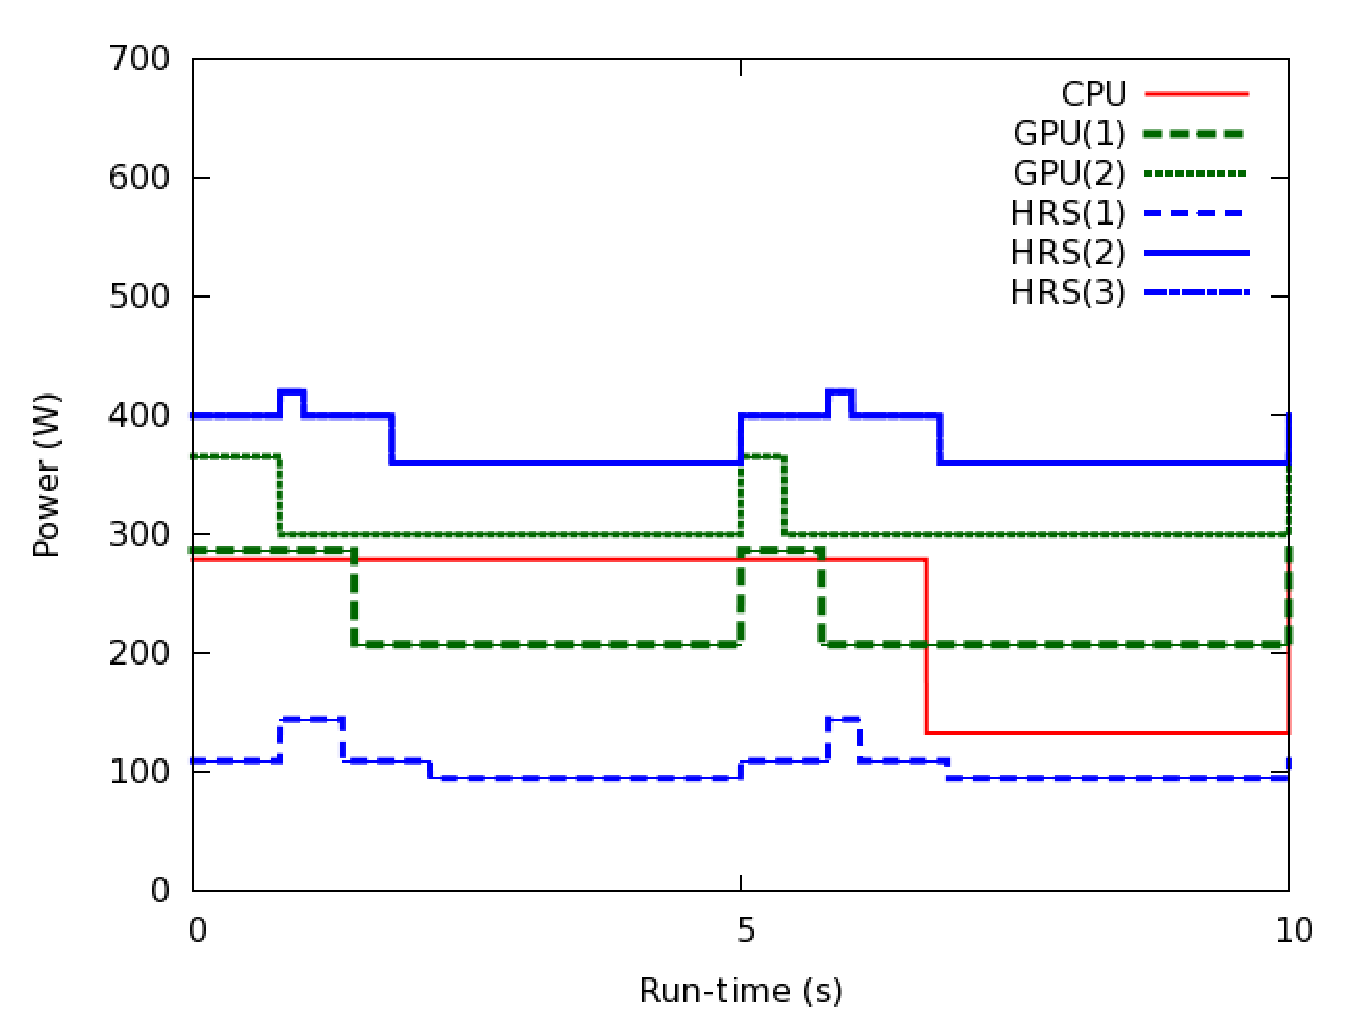
\includegraphics[width=0.7\textwidth]{runtime_reconfiguration/figures/fig_power2}
\caption{Power consumption of HRS, CPU and GPU in one time-step, notice that the computation time of the CPU system exceeds the 5-second real-time requirement (The lines of HRS(2) and HRS(3) overlap)}
\label{fig:power}
\end{figure}

To identify the speed and energy trade-off, we produce a graph as shown in Figure~\ref{fig:scale}. 
Each data point represents the computation time versus energy consumption of a system setting.
Among all the systems, the HRS with one FPGA has the computation speed that satisfies the real-time requirement, while at the same time consumes the smallest amount of energy.
All the configurations of CPU system cannot meet the real-time requirement.
HRS(3), the HRS with four FPGAs, is the fastest among all the systems in comparison, therefore it is able to handle larger problems and more complex applications.

\begin{figure}[t!]
\centering
\includegraphics[width=0.7\textwidth]{runtime_reconfiguration/figures/fig_scale}
\caption{Run-time vs. energy consumption of HRS, CPUs and GPUs (5-second time-step, 67M particles; Refer to Table~II for system settings)}
\label{fig:scale}
\end{figure}


%%%%%%%%%%%%%%%%%%%%%%%%%%%%%%%%%%%%%%%%
\section{Summary}

This paper presents an adaptive particle filter for real-time applications.
The proposed heterogeneous reconfigurable system demonstrates a significant reduction in power and energy consumption compared with CPU and GPU.
The adaptive algorithm reduces computation time while maintaining quality of results. 
The approach is scalable to systems with multiple FPGAs.
A data compression technique is used to mitigate the data transfer overhead between the FPGAs and CPUs.

In the future, heterogeneous reconfigurable systems will be developed for other particle filters that are more compute-intensive and have more stringent real-time requirements.
Air traffic management~\cite{chau13b} and traffic estimation~\cite{mihaylova07} are example applications that can substantially benefit from the proposed approach in meeting current and future requirements.
Further work will also be required to automate the optimisation of designs targeting heterogeneous reconfigurable systems.


%%%%%%%%%%%%%%%%%%%%%%%%%%%%%%%%%%%%%%%%

